
\documentclass[11pt]{scrartcl}
\usepackage[latin1]{inputenc}
\usepackage[T1]{fontenc}
\usepackage[english]{babel}
\usepackage{graphicx}
\usepackage{textcomp}
\usepackage{setspace}

\usepackage{pdfpages}

\setlength{\parindent}{0cm}

\pagestyle{myheadings}
\markright{\tiny{DD - Signal Transmission, Version\,0.6, \today - (for TOBI internal use only, must not be published or distributed)}}

\begin{document}

  \begin{center}
  \textbf{\Large{TOBI - Hybrid BCI -- Data Transmission\linebreak \textit{Design Document}}\\  \vspace*{0.3cm}
                  \textcolor{red}{(for TOBI internal use only,\\ must not be published or distributed)} }\\
    \vspace*{0.2cm}
    TUG,\quad Graz, \today{}
  \end{center}


\section{Reqirements}
  \begin{itemize}
    \item \textbf{Combined signal data server (EEG, EMG, other signal types)}
    \newline
    \item Data transmission over network (or localhost) using NW-sockets
    \item Software should be platform independent (portable framework and libraries)
    \item Multiple clients possible
    \item Possibility against package leakage
    \item Hardware requirements low
    \item Configuration communication over Network
    \item Variable number of EEG/EMG/\dots channels
    \item Variable sampling frequency
    \item Variety of data acquisition hardware possible\\
      \hspace*{0.2cm} (EEG: at the beginning only g-tec USBAmp, EMG amplifier, joysticks,\dots)
    \item Delivery of data data ``in time''
    \newline
    \item Possibility to store data with higher sampling rate
      \hspace*{0.2cm} (internal downsampling before transmission)
    \item Connection oriented transfer (e.g. using TCP) with modified sampling rate
  \end{itemize}

\section{Client - Server Architecture}
  \begin{itemize}
    \item One data server
    \item ``Many'' clients
    \item Clients can be attached to the server at any time
    \item Communication seperated into ``configuration communication'' and data transmission
    \item Server provides one TCP socket for ``configuration communication''
    \item ``Configuration communication'' done in xml-style
    \item Server provides one UDP socket for data broadcast\\
      \hspace*{0.2cm} (packet loss acceptable)
    \item Server provides one TCP socket for connection oriented data transmission\\
      \hspace*{0.2cm} (packet loss \textbf{un}acceptable)
    \newline
    \item Clients create connections to respective server socket
    \item Data transmission to multiple clients done by broad- or multicast
  \end{itemize}

\section{Startup and Connection-Setup -- an idea}

  Before any network activity:
  \begin{itemize}
    \item Server starts with HW configuration and UDP/TCP ports specified in .xml file
    \item Client starts with configuration in .xml file\\
      \hspace*{0.2cm} (server-IP and ports are familiar to the client)
  \end{itemize}

  All network-messages are in xml-style, except data\\
  UDP packets will be broadcasted into the whole subnet.\\

  Connection scheme shown in Figure\,\ref{fig:client-server}.


  Client-Server handshake shown in Figure\,\ref{fig:handshake}.

    \begin{figure}[htb]
      \centering
        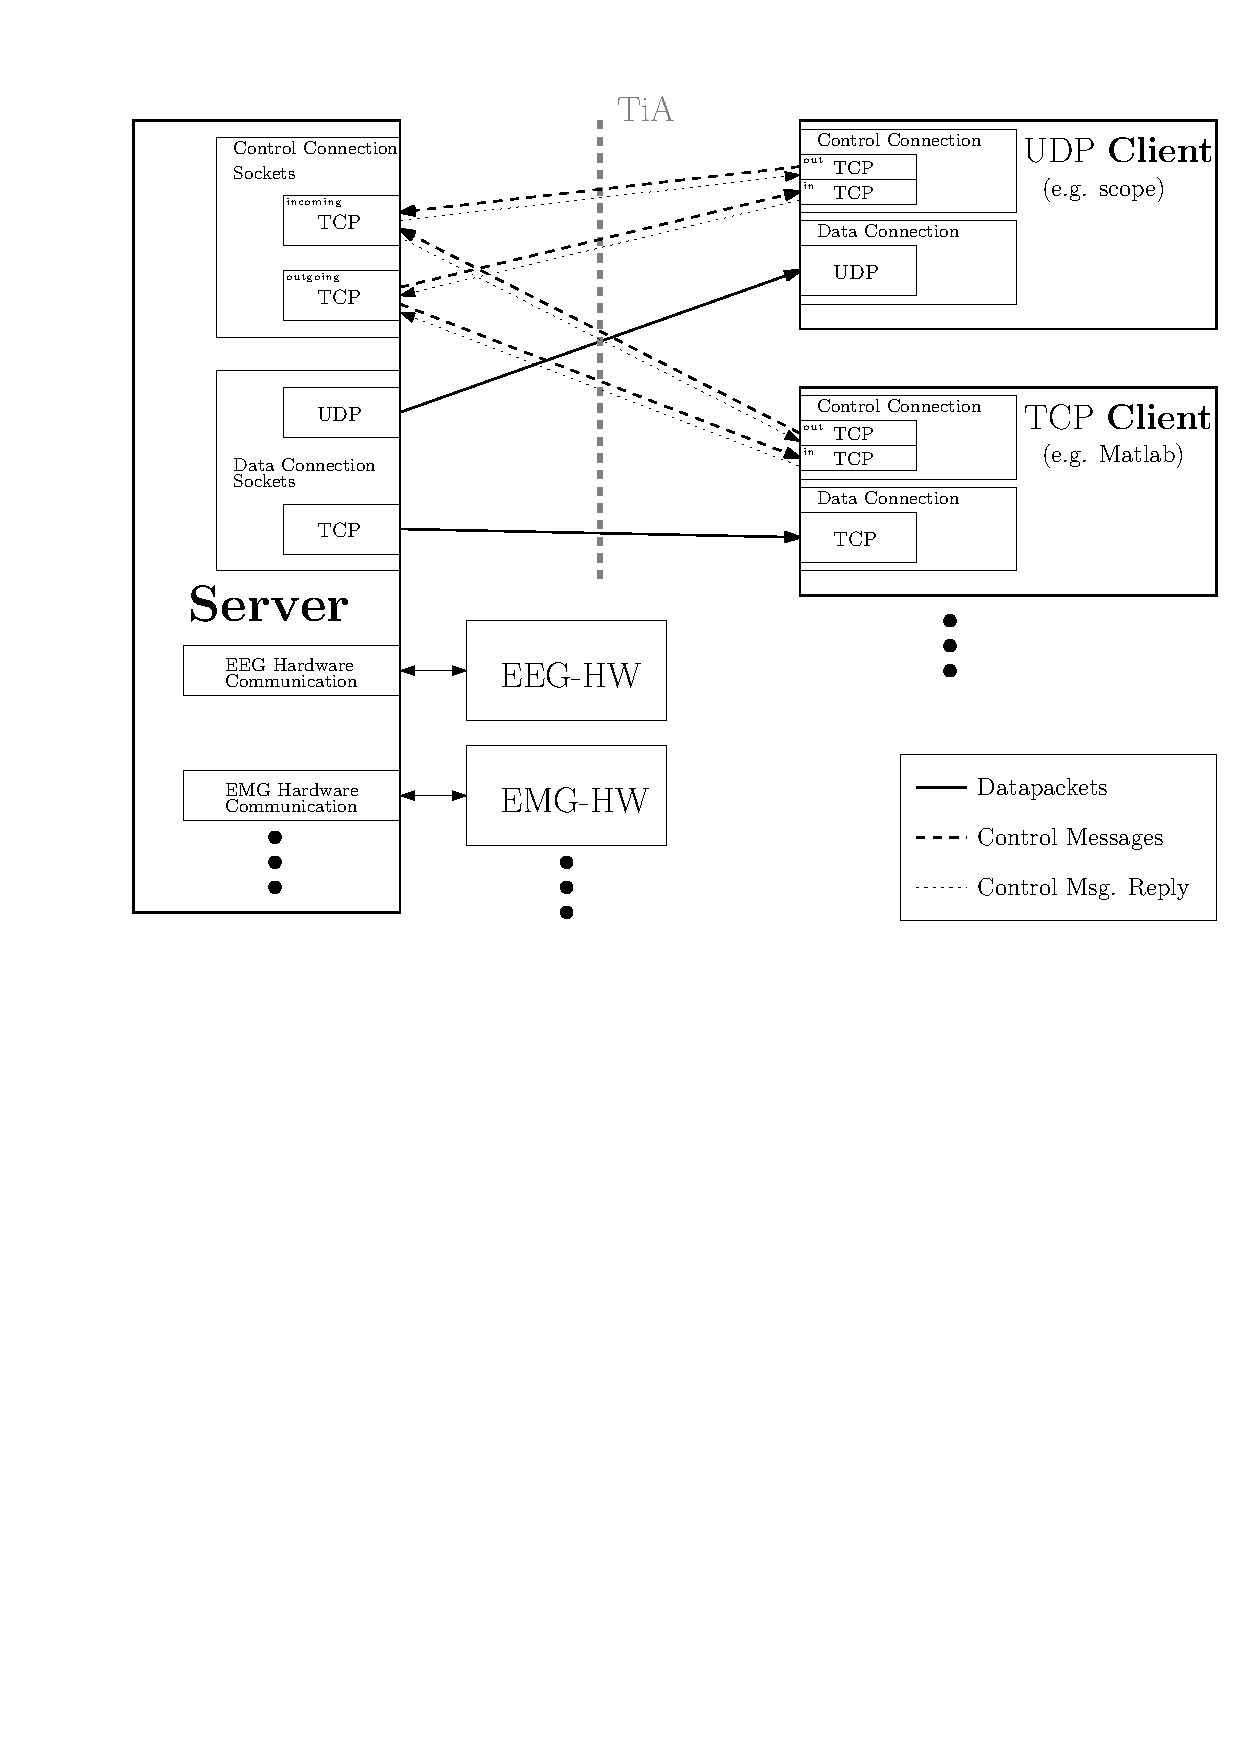
\includegraphics[scale=0.7]{Client-Server.pdf}
      \caption{Connection Scheme Client-Server}
      \label{fig:client-server}
    \end{figure}

    \begin{figure}
      \centering
        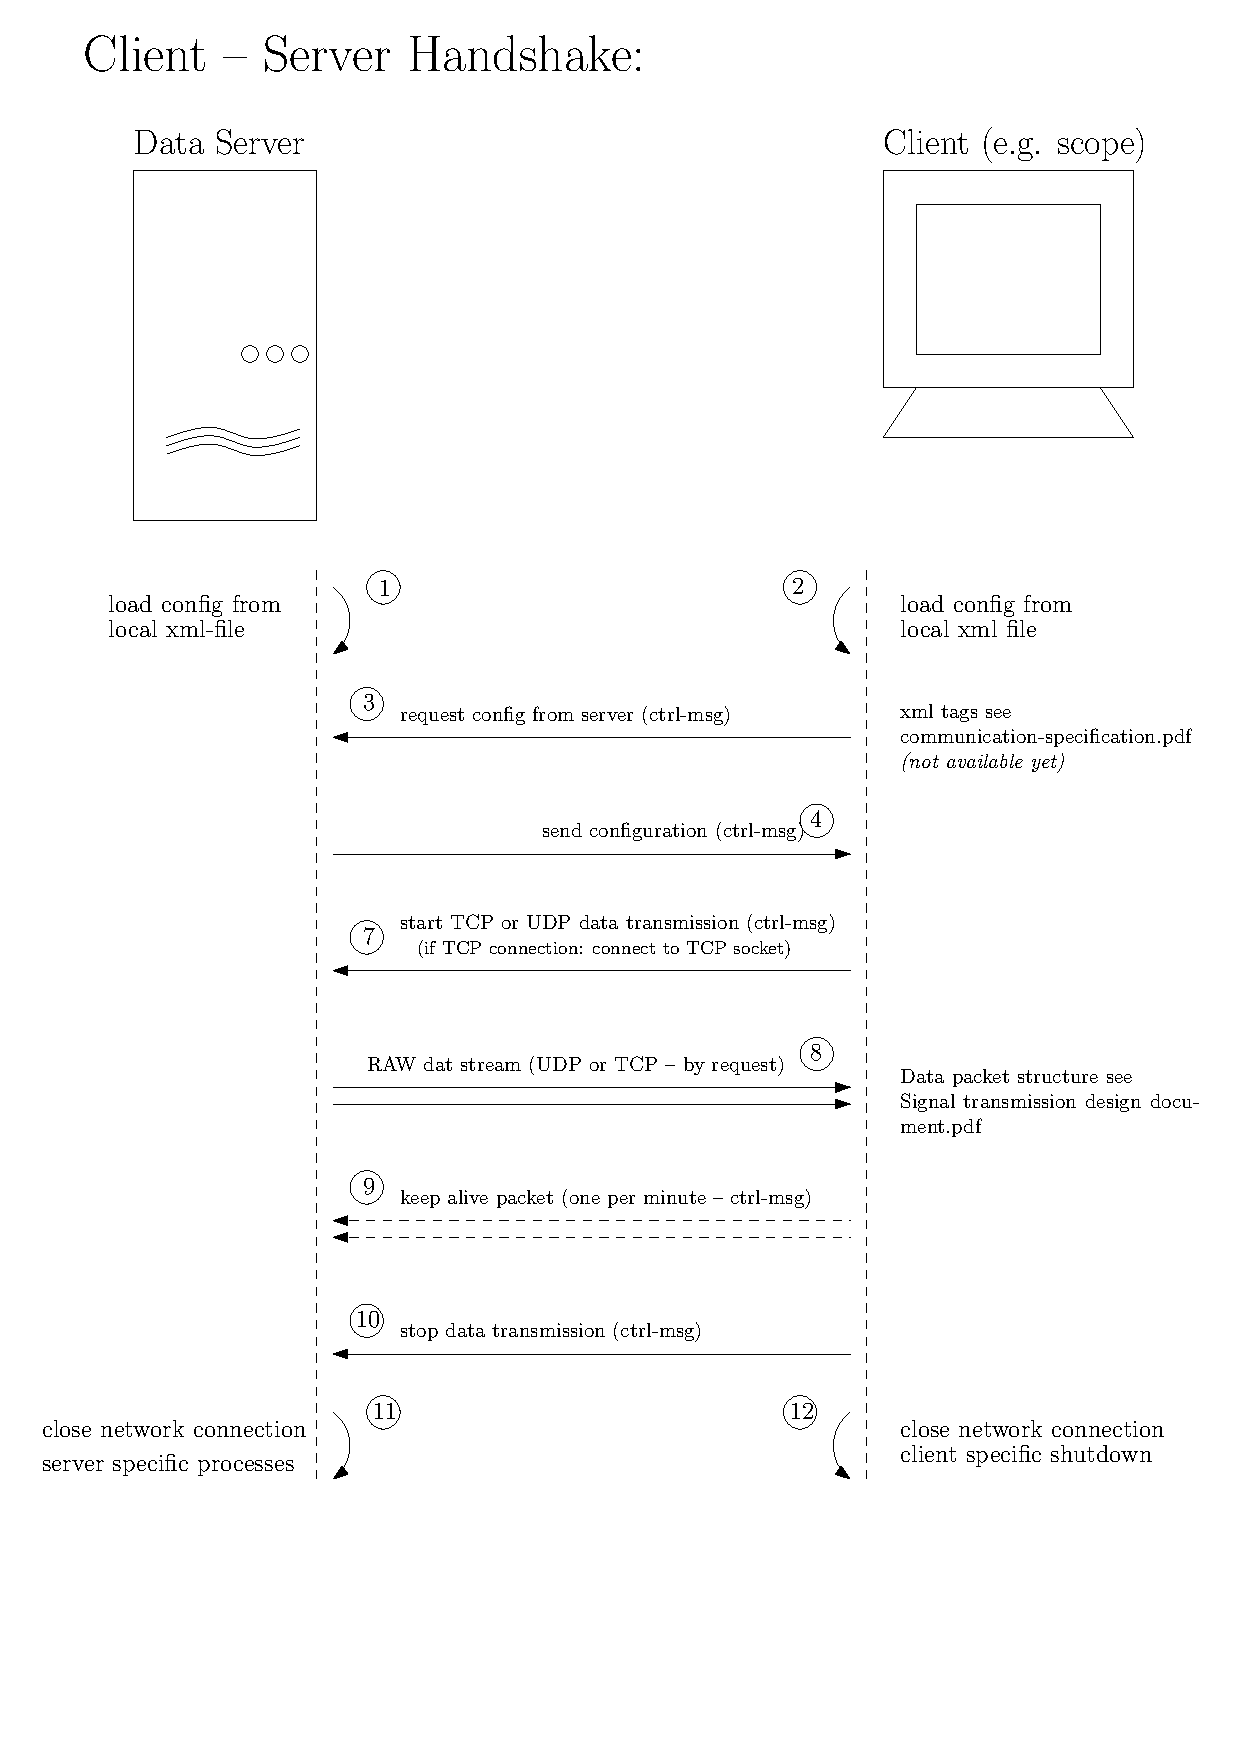
\includegraphics[scale=0.7]{Client-Server-Handshake.pdf}
      \caption{Client-Server Handshake}
      \label{fig:handshake}
    \end{figure}

  \begin{itemize}
%     \item Automatic HW-detection possible (generate List of hardware)
    \item Client connects to server and requests configuration\\
      \hspace*{0.2cm} (sampling rate, nr. of channels, stored signal data type (int, float,\dots))
    \item Server sends configuration
    \item Client requests start of UDP or TCP data transmission\\
      \hspace*{0.2cm} (data loss unacceptable $\rightarrow$  data over TCP connection\\
      \hspace*{0.2cm} ~if TCP connection: connect to server TCP socket)
    \item Server starts data transmission
    \newline
    \item Optional: Other Clients connect to the server
    \newline
    \item Client requests to stop data stream
    \item UDP: if other clients available: keep transmitting data\\
          TCP: stop transmitting data over TCP connection
    \item Client closes connection to server (client specific shutdown)
    \item Last clients requests to stop data stream
    \item Server closes connection to last client and stops transmitting data
    \item Client specific shutdown
  \end{itemize}

\section{The Connection -- TCP, UDP, creation, termination, \dots}

  \begin{itemize}
    \item Protocol application dependent\\
      \quad (UDP for scope, TCP for critical apps \dots data loss unacceptable)
    \item Data stream can't stop while clients are attached
    \item Configuration done by xml files
    \item Communication between client and server done in xml-style
  \end{itemize}

\clearpage

\section{The Packet -- what's inside}

  \underline{Header}:
  \begin{itemize}
    \item Flags
    \item Running Packet Number $\rightarrow$ loss of data can be recognized
    \item Running Sample Number\\
      \hspace*{0.15cm}$\rightarrow$ if transmitting with different sampling rates, related\\
      \hspace*{0.5cm} samples can be clearly identified
    \item Number of different signal types $\rightarrow$ loss of data can be recognized
    \item Offset of signal types in the packet
    \item Number of channels per signal type
  \end{itemize}

  \underline{Data:}
  \begin{itemize}
    \item EEG (RAW values -- type EEG amplifier specific)
    \item EMG (RAW values -- type EEG amplifier specific)
    \item Other Signal types (ECG, manual input e.g. button)
    \newline
    \item if needed also Events
    \item Additional Information ?? (again Channels, Frequency,\dots)
  \end{itemize}
  
  \vspace*{0.5cm}
  Data will be sent either as floats (4\.byte) or doubles (8\,byte). The biggest type, dependent on the data acquisition system will be chosen for all transmitted data.\\
  For scaling purposes, all equal signals have to scaled to the same range (e.g. \textmu V, mV,\dots).\\
  \\
  \textbf{Defined Flags and data order:}\\
  \hspace*{0.3cm} $\rightarrow$ Signals in predefined order:\\
  \hspace*{0.6cm} EEG   |   EMG   |   EOG   |   ECG   |   HR    |   BP    |   Buttons   |   Joystick    |   Sensors   |   \ldots \\
  \\
  \hspace*{0.3cm} \underline{32 bit flags:}
  \begin{itemize}
    \item[01]  \ldots EEG (0x0001)
    \item[02]  \ldots EMG (0x0002)
    \item[03]  \ldots EOG (0x0004)
    \item[04]  \ldots ECG (0x0008)
    \item[05]  \ldots HR  (0x0010)
    \item[06]  \ldots BP  (0x0020)
    \item[07]  \ldots Buttons  (0x0040)
    \item[08]  \ldots Joystick (0x0080)
    \item[09]  \ldots Sensors  (0x0100)
    \item[10]  \ldots NIRS     (0x0200)
    \item[11]  \ldots FMRI     (0x0400)
    \item[12]
    \item[13]
    \item[14]
    \item[15]
    \item[16]
    \item[17]  \ldots User Defined I    (0x010000)
    \item[18]  \ldots User Defined II   (0x020000)
    \item[19]  \ldots User Defined III  (0x040000)
    \item[20]  \ldots User Defined IV   (0x080000)
    \item[21]  \ldots UNDEFINED         (0x100000)
    \item[22]  \ldots Events            (0x200000)
    \item []
    \item[23]  \textbf{temporary RESERVED}: Packetcode (0x2400000) \ldots 1
    \item[24]  \textbf{temporary RESERVED}: Packetcode (0x2400000) \ldots 0
    \item[25]  \textbf{temporary RESERVED}: Packetcode (0x2400000) \ldots 0
    \item[26]  \textbf{temporary RESERVED}: Packetcode (0x2400000) \ldots 1
    \item []
    \item[27]  \textbf{RESERVED}: 6 bits for Packet Version
    \item[28]  \textbf{RESERVED}: 6 bits for Packet Version
    \item[29]  \textbf{RESERVED}: 6 bits for Packet Version
    \item[30]  \textbf{RESERVED}: 6 bits for Packet Version
    \item[31]  \textbf{RESERVED}: 6 bits for Packet Version
    \item[32]  \textbf{RESERVED}: 6 bits for Packet Version
  \end{itemize}

  \newpage

  Data packet structure shown in Figure\,\ref{fig:data-packet-structure}.\\

    \begin{figure}[htbp]
      \centering
        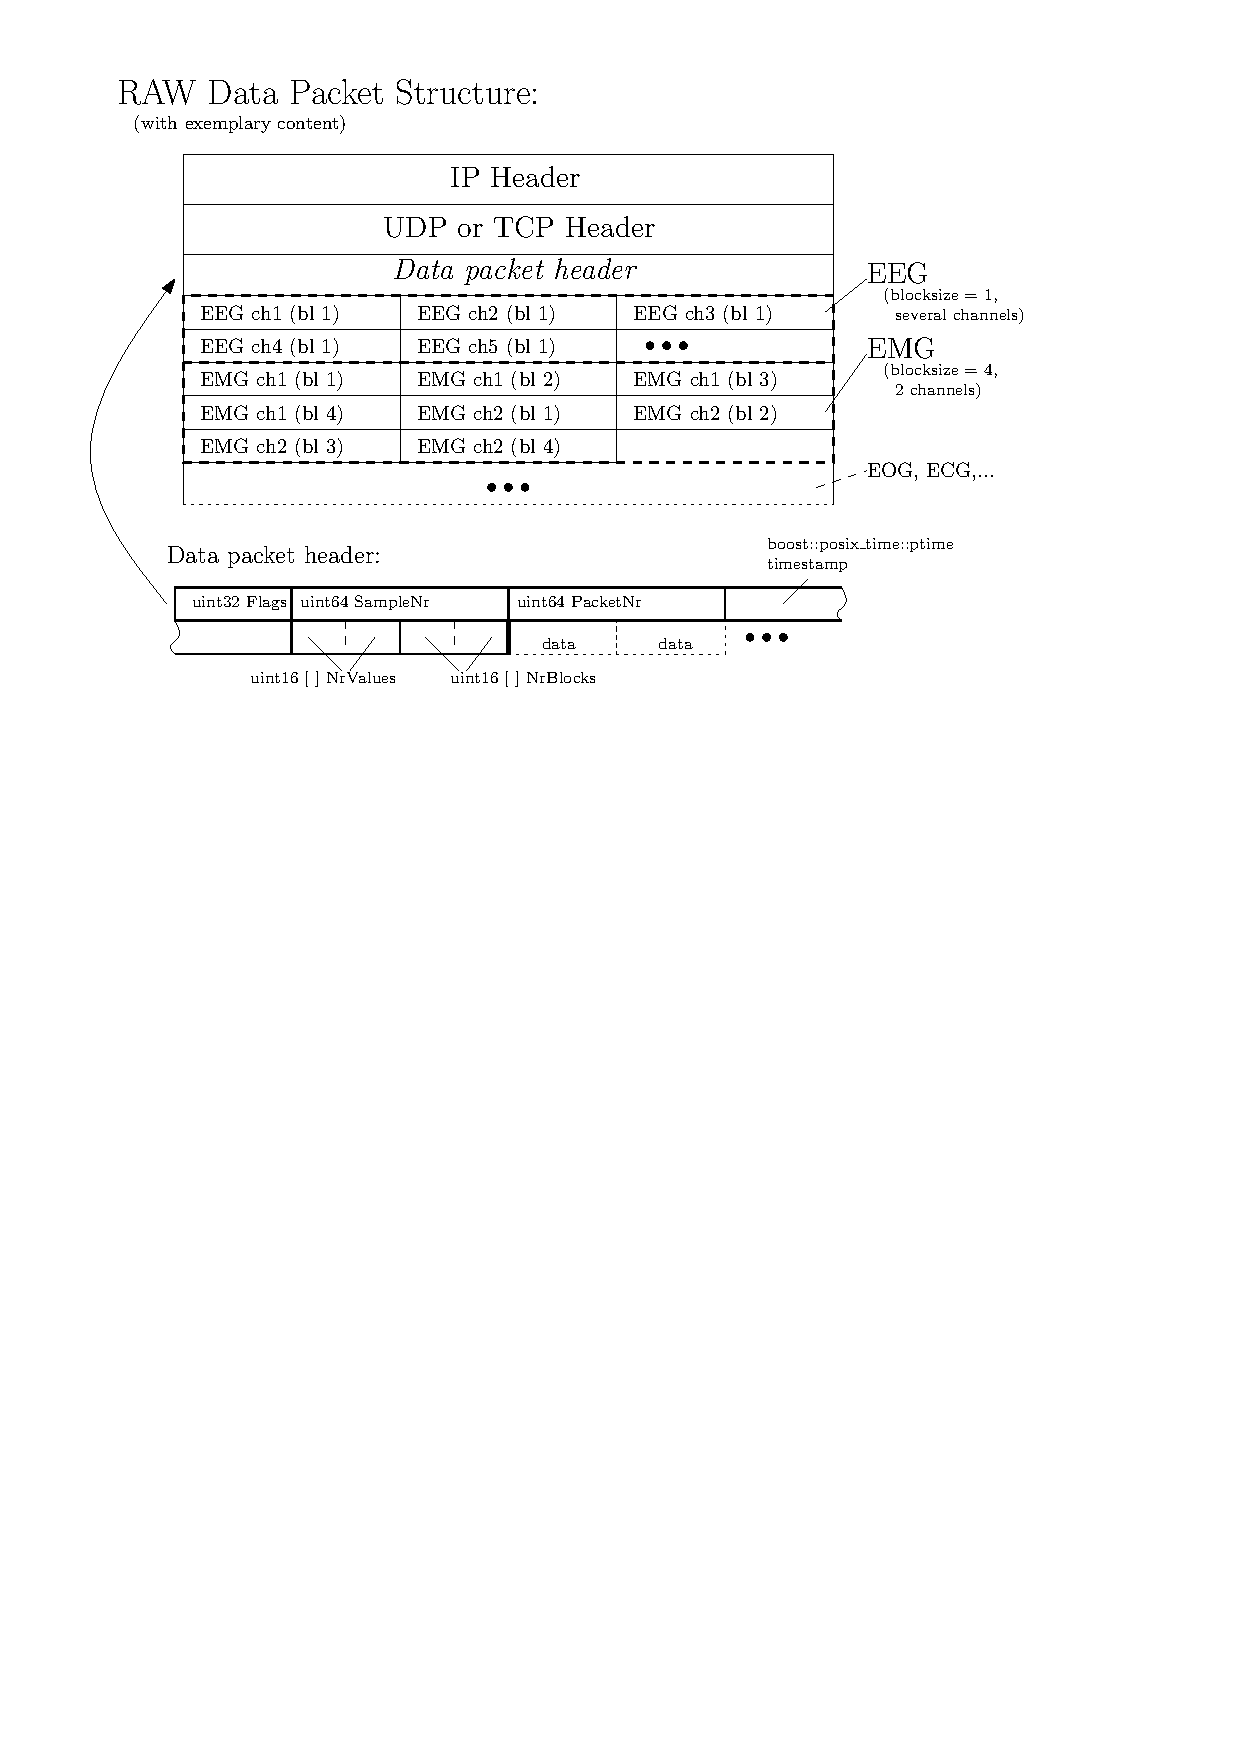
\includegraphics[scale=0.94]{data-packet-structure.pdf}
      \caption{data packet structure}
      \label{fig:data-packet-structure}
    \end{figure}

  \newpage
  \subsection{Estimation of needed bandwidth:}

  \underline{High values, overhead not included:}\\
  \\
  Sampling Rate $f_s$ = 512\,Hz\\
  Nr. of channels: n = 128\\
  Needed memory per channel and packet: s = 8 byte (double)\\

  \begin{displaymath}
    B = f_s \cdot (n + 1) \cdot s \quad = \quad 516\, \frac{kbyte}{s}
  \end{displaymath}
  \\

  \underline{Expected values, overhead not included:}\\
  \\
  Sampling Rate $f_s$ = 256\,Hz\\
  Nr. of channels: n = 16 (USBAmp)\\
  Needed memory per channel and packet: s = 8 byte (double)\\

  \begin{displaymath}
    B = f_s \cdot (n + 1) \cdot s \quad = \quad 34\, \frac{kbyte}{s}
  \end{displaymath}
  \\
  Within this calculations the packet overhead is not taken into account!

\section{Outcome -- WP5 and WP8 Meeting Berlin 7.7.09}
  \begin{itemize}
    \item Broadcast over UDP
    \item No realtime network protocol\\
      \hspace*{0.2cm} (until a rationale of need)
    \item Header to describe package content
    \item Combined server
    \item Offline simulation possible -- by loading an existing data file
    \item Downsampling for individual TCP connections done by the server
    \item Events transmitted by the data server
    \item Signal and event storage done by the server (use of .gdf format if possible)
    \item Different sapmling rates provided by the server
    \newline
    \item Differing package content described by data packet header (flags, offsets,\dots)
    \item Storage with higher sampling rate than transmission possible
  \end{itemize}

\section{Discussion Points}

  \textbf{Discussed:}
  \begin{itemize}
    \item Additional requirements? (use of shared memory for communication)
    \item More than one client over UDP \dots broadcast or multicast?? (preferably broadcast into subnet)
    \item Realtime protocol required?\\
      \hspace*{0.2cm} (250\,Hz \dots $\frac{1~packet}{4\,ms}$, mean RTT in small subnet ca. 0.5\,ms,\\
      \hspace*{0.2cm} ~maybe use of own 192.168.xxx.xxx subnet on a 2$^{nd}$ network interface card)
    \item Additional information in data packet
    \item Offline simulation needed (file with events and different signals sent by the server)
    \item Support of different sampling rates by the data server needed?\\
      \hspace*{0.2cm} (Problem: Increases network load, higher complexity, data packet structure)
    \item Event transmission/creating -- where/how?
    \item Data storage? -- where, how (EEG synchronisation with events)
    \item Different sapmling rates
  \end{itemize}

\textbf{Still open:}
  \begin{itemize}
    \item Definition of xml tags (partly done -- 13.4.2010)
    \item Preprocessing: done by the server or elsewhere? (additional to downsampling?)
    \item How to handle broken TCP connections? (client hang-up,\dots $\rightarrow$ keep-alive packet?)
  \end{itemize}
\end{document}
